\documentclass{paper}
\usepackage[utf8]{inputenc}
\usepackage{amsmath}
\usepackage{amsfonts}
\usepackage{amssymb}
\usepackage{amsthm}
\usepackage{graphicx}
\usepackage{wrapfig}
\usepackage{makecell}
\usepackage{xspace}
\usepackage[usenames,dvipsnames]{xcolor}
\usepackage{caption}
\usepackage{wrapfig}
\usepackage{float}
\usepackage{booktabs}
\usepackage[margin=0.7in,footskip=0.25in]{geometry}
\newtheorem{definition}{Definition}
\newtheorem{condition}{Condition}
\newtheorem{conjecture}{Conjecture}
\newtheorem{observation}{Observation}
\newtheorem{lemma}{Lemma}
\newtheorem{theorem}{Theorem}

\newcommand{\mremark}[3]{\textcolor{blue}{\textsc{#1 #2:}} \textcolor{SeaGreen}{\textsf{#3}}}

\newcommand{\frank}[2][says]{\mremark{Frank}{#1}{#2}}
\newcommand{\maarten}[2][says]{\mremark{Maarten}{#1}{#2}}
\newcommand{\marc}[2][says]{\mremark{Marc}{#1}{#2}}
\newcommand{\jerome}[2][says]{\mremark{J\'er\^ome}{#1}{#2}}
\newcommand{\jordi}[2][says]{\mremark{Jordi}{#1}{#2}}
\newcommand{\ivor}[2][says]{\mremark{Ivor}{#1}{#2}}
\newcommand{\todo}[2][DO]{\mremark{TO}{#1}{#2}}
\newcommand{\draw}{\todo{draw}}

\newcommand{\bigo}{\ensuremath{\mathcal O}}

\newcommand{\spg}{\mathcal{S\!P}}
\newcommand{\ixi}{\mathcal{I}}
\newcommand{\pix}{\resizebox{2mm}{2mm}{\square}}
\newcommand{\spix}{\boxplus}

\newcommand{\eps}{\varepsilon}
\newcommand{\R}{\mathbb{R}}

\title{Pixelating Polygons}
\begin{document}
\maketitle

\section{Introduction}

Given a set of simple polygons $\cal A$, we wish to assign each $A \in \cal A$ to a grid polygon (defined formally in Section~\ref {sec:prelims}) $X$ which represents $A$.


%To successfully map a disjoint hole $h_i$ we need to outline its border as a disjoint cycle of black cells.

%Now suppose that for two holes $h_1, h_2 \in H$ their border is present in the same cell $\pix \in G$. We could color the cell black, and say that the pixel is part of both the border of $h_1$ and of $h_2$. But in this case, the holes $h_1$ and $h_2$ intersect one another, whereas in the original drawing $A$ this was not the case. The only option that we have, is to stretch and transpose $A$, such that only one of the two holes has its border in $\pix$.

One way to measure how much we needed to "stretch" the original polygons is to measure the symmetrical Hausdorff distance between $A_i$ and its mapping $X_i$. 
We require that the Hausdorff distance between the boundaries of the polygons is limited and also that the Hausdorff distance between the points inside the polygons is limited.
Let $\eps$ be the maximum allowed Hausdorff distance, called \emph{stretch}.
\maarten {What is the intuition behind the use of the word "stretch" here? I would juse say "similarity" (or distance, or something like that).}

\iffalse
Formally this means: $\forall i\in \{1, m\}$
\begin{itemize}
	\item $\forall s\in \partial A_i, \exists t\in \partial X_i, |st|\leq \eps$
	\item $\forall s\in \partial X_i, \exists t\in \partial A_i, |st|\leq \eps$
	\item $\forall s\in  A_i, \exists t\in  X_i, |st|\leq \eps$
	\item $\forall s\in  X_i, \exists t\in  A_i, |st|\leq \eps$
\end{itemize}
where $|\cdot|$ denotes Euclidean distance.
\fi

The goal of this paper is to find a mapping where the stretch factor is asymptotically minimized. In this work we look at different types of polygons and the theta-bounds on the Hausdorff distance. See the table below for a summary of the results.
See Figure \ref{fig:pixelexample} for an example.

%\begin{definition}
%Suppose $H$ is a collection of holes $h_1 ... h_m$. Let $b_1 ... b_m$ be the borders of $h_1 ... h_m$ and let $f(H)$ be the projection of $H$ onto the grid.

%We say the projection $f$ is \textbf{valid} if there is a bijection $g$ between $\{ b_1 ... b_m \}$ and a set of disjoint black cycles in $f(H)$.
%\end{definition}

%\begin{lemma}
%\label{lemma:expand}
%\jerome{This is wrong!!!} \jerome{It is rather that for each grid polygon that we create, this holds.}
%Let $H$ be a collection of holes. If there exists a valid projection $f$, where for each border $b_i$, the symmetrical Hausdorff distance between $b_i$ and $g(b_i)$ is $\Theta( X)$, then the symmetrical Hausdorff distance between $H$ and $f(H)$ is $\Theta(X)$.
%\end{lemma}

%This lemma allows us to focus on only projecting the boundaries of a hole.


%\begin{figure}[H]
%\centering
%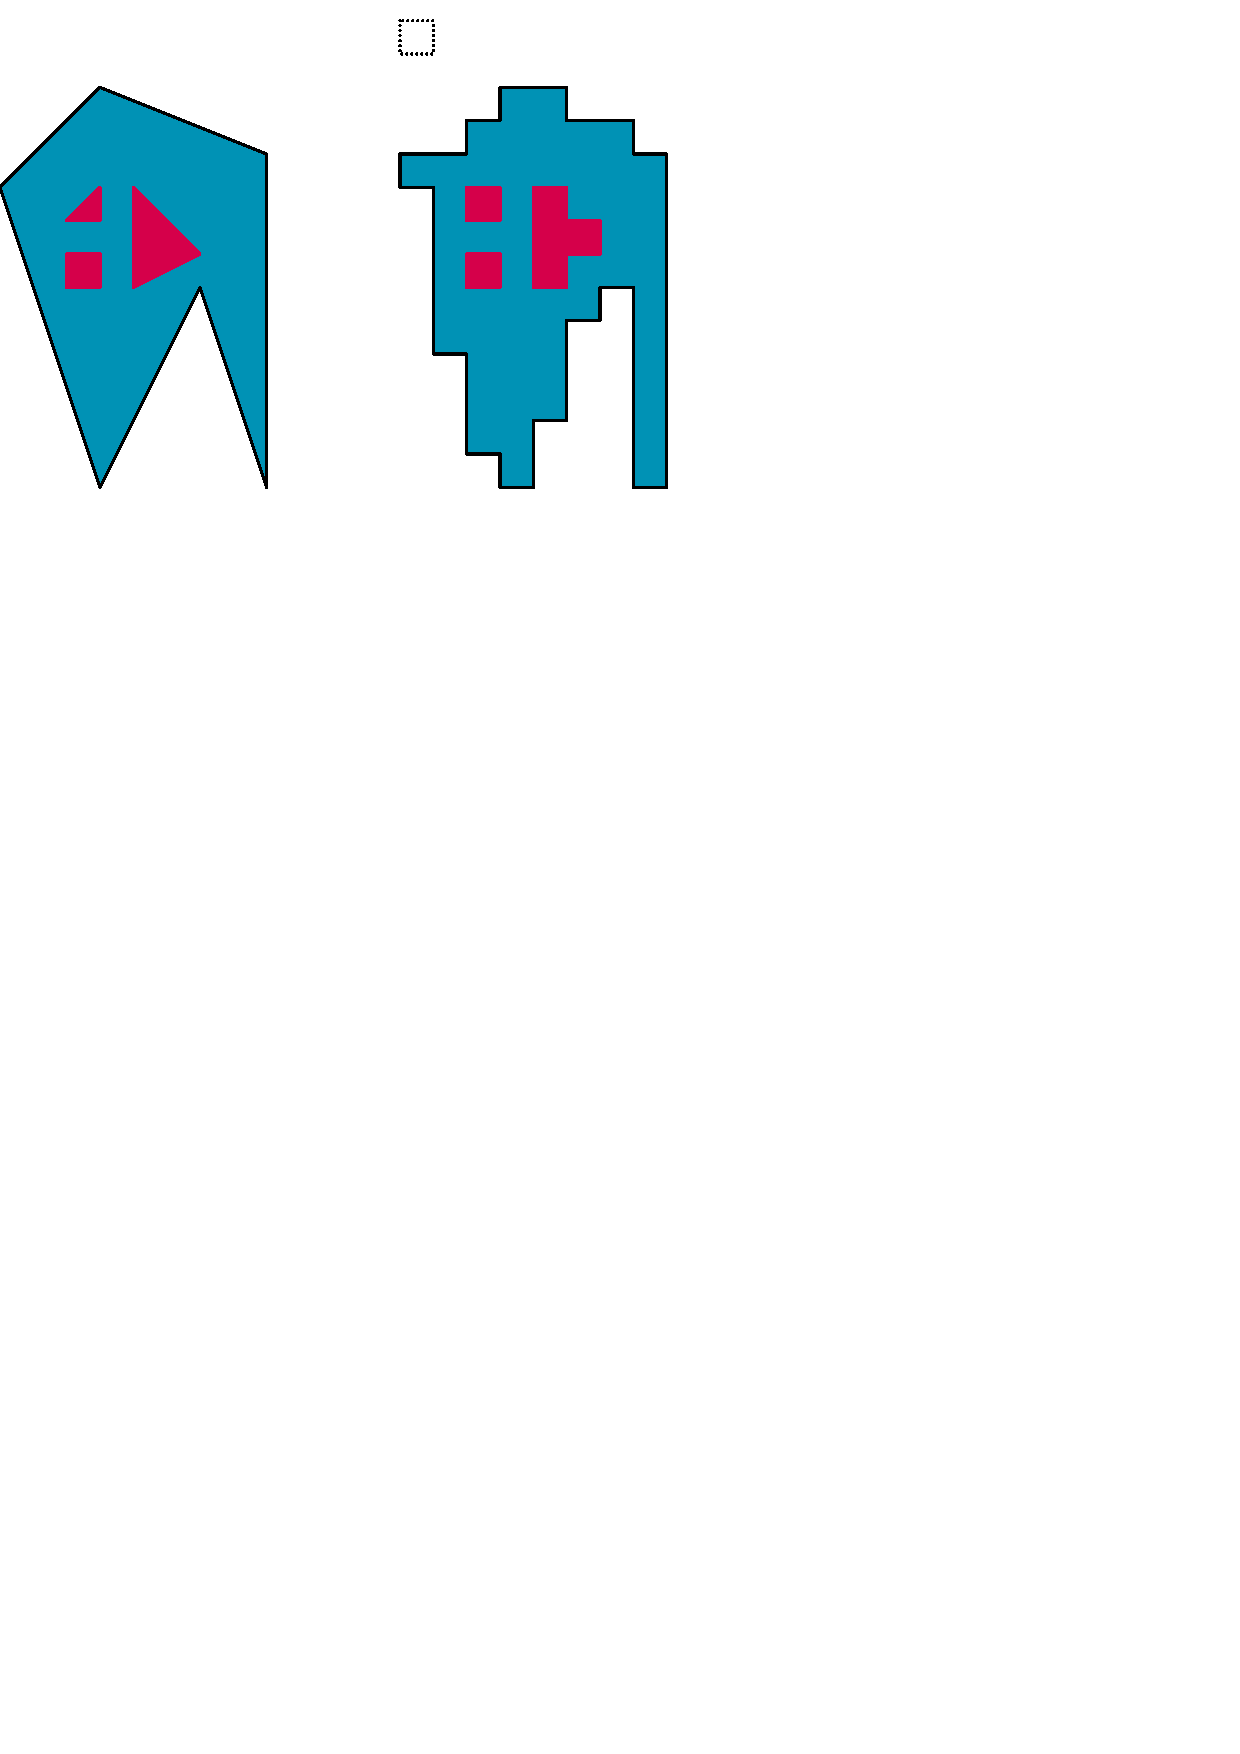
\includegraphics[width=150px]{Figures/pixelexample.pdf}
%\caption{\jerome{redo}
%Left is $A$: A simple polygon with $m=3$ holes. To the right is the projection $B$ to pixels with diameter $d$ with a symmetrical Hausdorff distance less than $2*d$.
%}
%\label{fig:pixelexample}
%\end{figure}




\begin{table}[H]
\begin{tabular}{lcc}
\toprule
Restrictions on the polygons & Lower bound & Upper bound  \\ \midrule
Polygons are points & $\Omega(\sqrt[]{m}) $ & $\bigo(\sqrt[]{m})$ \\
Polygons are $\beta$-fat regions & $\Omega(\sqrt[]{m}) $ & $\bigo(\sqrt[]{m})$ \\
Polygons are convex regions & $\Omega(m) $ & $\bigo(m)$ \\
Two polygons without restrictions &  $\Omega(1)$ & $\bigo(1)$\\
Three polygons without restrictions &  \multicolumn{2}{c}{unbounded}\\
\bottomrule
%$\Omega(2^m)$ & $\bigo(2^m)$ \\ \hline
\end{tabular}
\end{table}


\section{Preliminaries}

\paragraph {Simple grid polygons.}

Let $\Xi$ be the (infinite) unit grid, which we interpret as a set of {\em pixels} (unit squares): an element $\pix \in \Xi$ is a subset of $\R^2$ of the form $[a,a+1]\times[b,b+1]$ for integers $a$ and $b$.
For a given set of pixels $X \subset \Xi$, we denote the region $\cup_{\pix \in X}\pix$ covered by $X$ simply by $\cup(X)$, and we write $\partial(X)$ for the boundary of $\cup(X)$.

\begin{definition}
A {\em simple grid polygon} is a set of pixels $X \subset \Xi$ for which $\partial(X)$ is a single closed curve.
\end{definition}

\maarten {Not sure we need the following definitions.}

\begin{definition}
Two pixels are \emph{adjacent} iff they share a side.
\end{definition}

Adjacency induces the graph $G=(\Xi, E)$ with $(v, w)\in E \iff v$ and $w$ are adjacent.
For $v\in \Xi$, let $N(v)$ be the four neighbors of v. Further for $W\subseteq \Xi$, let $N(W)=\bigcup_{v\in W} N(v)$.

\paragraph {Similarity.}

The {\em Hausdorff distance}~\cite{} between two sets $A, B \subset \R^2$ is defined as 
\[
  H(A, B) = \max \{\max_{a \in A}(\min_{b \in B}(|ab|)), \max_{b \in B}(\min_{a \in A}(|ab|))\}$
\]

Note that the Hausdorff distance between any two closed sets is equal to the Hausdorff distance between the boundaries of those sets.

Let $A$ be a simple polygon (with real-valued coordinates), and let $X$ be a simple grid polygon.

\begin{definition}
We say $A$ and $X$ are {\em $\eps$-similar} if $H(A,\partial(X)) \le \eps$. 
\end{definition}


\paragraph {Problem statement.}

Consider a set of $m$ simple polygons $\mathcal{A} = \{A_1, A_2, \ldots, A_m\}$ in $\mathbb{R}^2$ with $n$ vertices in total.
We wish to assign to each $A_i$ a distinct subset $X_i$ of $\Xi$ such that $X_i$ is a simple grid polygon and $X_i$ is $\eps$-similar to $A_i$.
We further require that the grid polygons are sufficiently spaced; that is, $\partial(X_i) \cap \partial(X_j) = \emptyset \forall i \ne j$. \maarten {Do we? Or do we only require the actual sets of pixels to be disjoint? It doesn't really matter, so what we do depends on the story we tell in the introduction, I think.}

\maarten {The following is an equivalent interpretation of the problem, which could help with the intuition and/or be used in the technical sections. If we don't use it, we might not want to define it.}

We may interpret a solution as a {\em coloring} of $\Xi$ in the following way.
Each pixel $\pix\in\Xi$ can only be assigned one color. The set of colors is $C = \{c_1,\dots c_m\}\cup\{b\}$, where $c_i$ is the color of the input polygon $A_i$ and $b$ is the background color.
Formally the coloring is then a map $f:\Xi\to C$.
Let ${\cal X}_f=\{X_1,\dots, X_m\}$ or short ${\cal X)$ be the set of grid polygons induced by $f$.

\begin{definition}
A coloring is \emph{valid}, iff the following holds:
\begin{enumerate}
	\item When two adjacent pixels have a different color, the one of them must be $b$. That way no two polygons touch.
	\item For each polygon $h_i$ the pixels colored $c_i$ is simple. Let $p_i$ be the polygon formed by those pixels.
	\item The polygon $p_i$ formed by the pixels colored does not contain holes.
\end{enumerate}

%If we want to use the same definition as Bouts~\emph{et al.}, we also request that the pixels on the boundary of $p_i$ form a simple cycle without chords. Informally this means that $p_i$ does not contain holes.
%\jerome{But that way we can have a rectangle + one pixel, because the boundary is then a cycle with a leaf\dots (???)}
\end{definition}


\paragraph {Superpixels.}

The following concepts will be useful.

\begin{definition}
%In all of the following chapters we use the following notion:
A \emph{superpixel} $\spix$ of size $k^2$ is a set of $k^2$ pixels forming a square with side length $k$.
A superpixel grid of size $k^2$ is a set $\spg$ of superpixels of length $k$ each such that the following holds:
(1) each pixel is in exactly one superpixel,(2) the superpixels are aligned, i.e., $\forall \spix_1, \spix_2\in \spg, |N(\spix_1)\cap \spix_2| \in \{0, k\}$.
\end{definition}

The superpixels induce the graph $G$ is the same way that the pixels induce $G$.

For a pixel $\pix$ we denote by $a(\pix)\in \mathbb{R}$ the set of points covered by $\pix$. Similarly for a superpixel $\spix$ we denote by $a(\spix)$ the set of points covered by the pixels in $\spix$. A polygon $q$ \emph{intersects} (super)pixel $o$ if $q\cap a(o)\neq \emptyset$. A polygon $q$ \emph{contains} (super)pixel $o$ if $a(o)\subseteq q$. 

\begin{definition}
For a fixed $i\in \{1, m\}$ and a valid coloring $C$ of $A$ using the pixels of $S$ and a given superpixel grid $\spg$, the polygon $p_i$ \emph{respects} $\spg$, if the following holds for each $\spix\in \spg$:
\begin{enumerate}
	\item if $h_i$ contains a superpixel, then so does $p_i$ and vis-versa,
	\item if $h_i$ intersects a superpixel, then so does $p_i$ and vis-versa.
\end{enumerate}
\end{definition}

\begin{lemma}\label{lem:respect_means_bound}
Let $A$ be a set of input polygons, $S$ be the screen and $\spg$ a superpixel grid of size $k^2$. Further let $C$ be a valid coloring of $A$ using the pixels of $S$.
If each polygon in $P_C$ respects $\spg$, then the stretch of the coloring is at most $\sqrt{2}k$.
\end{lemma}
The proof follows by definition.

\section{Polygons are points.}
\label{sec:points}

TL;DR

lower bound:
place them all within one pixel

upper bound: worst case optimal algorithm

overlay everything with superpixels, and then place pixels at random

\subsection{Lower Bound}
\label{sub:points_lower}



% subsection points_lower (end)

\subsection{Constructive Upper Bound}
\label{sub:points_upper}



% subsection points_upper (end)

\subsection{(Algorithm)}
\label{sub:points_algo}



% subsection points_algo (end)



% section points (end)

\section{Polygons are convex $\beta$-fat regions.}
\label{sec:fat}
TL;DR

lower bound

same as above

upper bound

overlay everything with superpixels:
\begin{enumerate}
	\item if a SP is completely covered $\rightarrow$ color
	%\item for each poly that has superpixels, but they are not connected, connect them using SPs where the poly is present
	\item then for each poly not yet present at all: choose random pixel in a SP where you are.
\end{enumerate}
This means Lemma~\ref{lem:respect_means_bound} is not completely fulfilled. We did not make sure that each polygon $p_i$ is present in each SP that $h_i$ intersects. But due to the fatness, we know that we are at least present in a ~close-by SP. We just have to prove that this is a constant and then we are done using a proof similar to the lemma.


(Note that if the regions are not convex, then the polygons could be disconnected.)


\subsection{Lower Bound}
\label{sub:fat_lower}



% subsection fat_lower (end)

\subsection{Constructive Upper Bound}
\label{sub:fat_upper}



% subsection fat_upper (end)

\subsection{(Algorithm)}
\label{sub:fat_algo}



% subsection fat_algo (end)


% section fat (end)

\section{Polygons are convex regions.}
\label{sec:convex}

TL;DR

lower bound

Each polygon is a long vertical segment. The $m$ polygons all pass through the same pixels.

upper bound

The algorithm first reports for each superpixel which  polygons intersect it.

Then for each pair of polygons we determine whether there is a horizontal line intersecting both. This induces a partial ordering on the x-axis because they are convex.
We choose one arbitrary order respecting the partial ordering: $x: \{1, m\}\to \{1, m\}, i\mapsto x(i)$.
We then do the same for vertical lines thus creating: $y: \{1, m\}\to \{1, m\}, i\mapsto y(i)$.

Each superpixel has side length $2\times h+1$. The pixel $(2\times x(i), 2\times y(i))$ is colored $c_i$.

Then for each pair of adjacent SPs we check which polygons intersect it. For each such polygon $h_i$ we connect the two pixels in the two SPs using a straight lines of pixels.

Finally whenever four SPs forming a square all contain a certain color $c_i$, then we color the square formed by those pixel in.

Before we use Lemma~\ref{lem:respect_means_bound}, we need to prove that containment implies containment, but that is easy with the step above.

qed


\subsection{Lower Bound}
\label{sub:convex_lower}

Let the polygons have as their only requirement that they are convex. In that case we can immediately show that the coloring has a lower-bound Hausdorff distance of $\Theta(m)$. The construction is shown in Figure \ref{fig:linesexample}.

\begin{figure}[H]
\centering

\includegraphics[width=20px]{Figures/linesexample.png}
\caption{The dotted square is a pixel. We can let $m$ vertical lines intersect the pixel. If their length is far greater than $m$, we can only project these regions to $m$ disjoint lines of pixels, which means that the outer lines must have a Hausdorff distance of $\Theta(m)$.}
\label{fig:linesexample}
\end{figure}


% subsection convex_lower (end)

\subsection{Constructive Upper Bound}
\label{sub:convex_upper}

\todo{expand}

We would like to create a projection of any set of convex Polygons $A$ that implements this lower bound such that all the projected regions are orthoconvex.



\begin{observation}
Let $h_1,h_2 \in A$ be two convex polygons. If there exists a horizontal line segment $l_1$ which intersects $h_1$ and $h_2$ such that on $l_1$, $h_1$ is left from $h_2$ then there cannot be another horizontal line segment $l_2$ which intersects $h_1$ and $h_2$ such that on $l_2$, $h_1$ lies to the right of $h_2$. A symmetrical property holds for vertical line segments if we look at which segment is higher.
\end{observation}

To explain our orthoconvex projection, we first introduce some notation: the observation allows us to create a partial order $P_x$ and $P_y$ based on intersections with horizontal and vertical line segments respectively. Let $\spg$ be a grid of superpixels with size $(2md+1)^2$. We define $X_A$ and $Y_A$ to be two indexes on $A$ that respect the partial orders $P_x$ and $P_y$ respectively. For any $\spix \in G$ we denote $spix[x,y]$ to be the pixel in $\spix$ that is the $2x$'th from the left and the $2y$'th pixel from the top. The algorithm involves assigning superpixels and pixels in $\spg$ to polygons and in the end connecting those polygons.

\begin{enumerate}
%\item If a hole $h$ covers at least one super pixel $D \in G$, we assign all $D$ which are coved by $h$ entirely to $h$.
%\item If a hole $h$ covers no super pixel, then for each super pixel $D$ which is intersected by $h$ we assign $D[X_H(h), Y_H(h)]$ to $h$.
\item For each superpixel $\spix$ which is intersected by a polygon $h$ we assign $D[X_H(h), Y_H(h)]$ to $h$.
\item For all polygons $h$, we connect all assigned pixels that are in adjacent superpixels with a horizontal and vertical line. 
\item If a set of lines encloses a region, we fill that region.
\end{enumerate}


\begin{figure}[H]
\centering
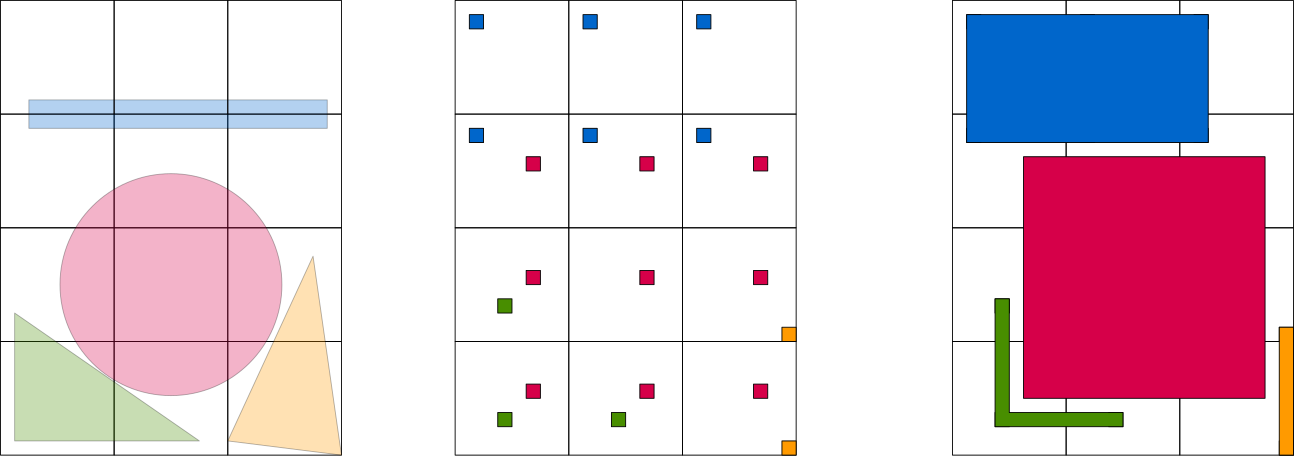
\includegraphics[width=400px]{Figures/convexprojection.png}
\caption{Four polygonss that intersect three times four superpixels and the steps of our algorithm.}
\label{fig:convexprojection}
\end{figure}

The result is clearly orthoconvex, since all assigned pixels are connected with horizontal and vertical lines and all enclosed regions are filled in. The result must also be disjoint: Any region that originally intersected a region which was filled in step 4 must originally have been to the left/right top/bottom of the region that filled a hole and thus is projected left/right above/below the filled region.


% subsection convex_upper (end)

\subsection{(Algorithm)}
\label{sub:convex_algo}



% subsection convex_algo (end)


% section convex (end)

\section{Arbitrary polygons.}
\label{sec:arbitrary}

\subsection{Two Polygons}

Refer to the paper "The painter’s problem: covering a grid with colored connected polygons".
Spoiler: we can pixelize two polygons at the same time using a constant stretch.

\subsection{Three of More Polygons}

\begin{theorem}\label{thm:unbouded}
The amount of stretch needed to color a screen with three or more polygons is unbounded.
\end{theorem}
\begin{proof}
Assume that the stretch needed to color a screen with three polygons is bounded by $k$.

Let $h_1$, $h_2$ and $h_3$ be three polygons defined as follows:
\jerome{spiral that loops around $k$ times.}

The area highlighted in Figure \todo{draw} is called $\ixi$.
Everything outside $\ixi$ can easily be drawn without much stretch.
% Also for everything outside $\mathcal{I}$, there is not much choice for the coloring (topologically). Area $\ixi$ is the problem here.
Note that at the top and the bottom we have $3k+3$ "connections" each. In $\ixi$ the pixels are colored in $c_1$ (red), $c_2$ (green) and $c_3$ (blue) such that in the end, the three polygons $p_1$, $p_2$ and $p_3$ induced by the three colors are connected.

%Let $\spg$ be a superpixel grid of size $f(\ell)$ \jerome{to be determined} aligned like in Figure~\draw. The input polygons $h_i$ intersect all of the superpixels in $\ixi$. \jerome{take care to make a small wiggle in the corners of the $\ixi$ so that this holds.}
%Just outside of $\ixi$ the superpixels blibla \todo{insert coordinates} all need to contain the colors redorgreenorblue.

Due to the choice of $\ixi$ we have that no pixel outside $\ixi$ and the loops is colored.
%Due to the choice of the size of $\spg$ we know that each pixel in any superpixel in the area highlighted in Figure~\draw is colored in the background color.
We assumed that the stretch was bounded by $k$, which implies that there is a valid coloring $C$ with stretch at most $k$.

Let $H=(W, F)$ be the Reeb graph of the (disconnected) polygon $R=(p_1\cup p_2\cup p_3)\cap \ixi$.
Note that $H$ is plane. Additionally $W$ contains $3\cdot k + 3$ vertices $W_t=\{r_1, g_1, b_1, r_2,\dots, r_{k+1}, g_{k+1}, b_{k+1}\}$ that correspond to the intersections of the polygons $p_1$, $p_2$ and $p_3$ and the top of $\ixi$. The names of the vertices indicate the color of the polygon. The vertices are sorted from left to right.
Similarly $W$ contains $3\cdot k + 3$ vertices $W_b=\textbf{}\{r'_0, g'_0, b'_0, r'_1,\dots, r'_k, g'_k, b'_k\}$ that correspond to the intersections of the polygons $p_1$, $p_2$ and $p_3$ and the bottom of $\ixi$.
Now if two vertices $r_i$ and $r_j$ are connected within $H$, then no vertex $g_e$ or $b_f$ that is between $r_i$ and $r_j$ can be connected to a vertex of $W_b$. Note that there are always at least two vertices of different color between two vertices of the same color in $W_t$.
Similarly we have that if two vertices $r'_i$ and $r'_j$ are connected, then the vertices $g'_e$ and $b'_f$ between $r'_i$ and $r'_j$ are not connected to any vertex of $W_t$.
And the same also holds for vertices of different color.

Now let $E$ be a connected component in $H$. Let $\{r_{i_1}, r_{i_2}, \dots, r_{i_e}, r'_{j_1}, \dots, r'_{j_f}\}$ be the members of $E$ that are in $W_t\cup W_b$, with $i_x<i_y$ and $j_x<j_y$. We say that $E$ contains $e-1$ \emph{top brackets} and $f-1$ \emph{bottom brackets}. If either $e$ or $f$ is non-zero, we say that $E$ contains a \emph{top-bottom connection}.

We know that when we remove $\ixi$ from the polygons $p_1$, $p_2$ and $p_3$, we obtain $3k+6$ polygons. If we do not remove $\ixi$ we have only three polygons. Therefore within $\ixi$ at least $3k+3$ connections (brackets and top-bottom connections) need to be made.
% This means that the connections within $\ixi$ must 
Now let $x$ (resp.\ $y$) be the number of top (resp.\ bottom) brackets over all connected components in $H$. Additionally let $z$ be the number of top-bottom connections over all connected components in $H$.
We already established that for each bracket there are at least two vertices of different color that can not be within a connected component with a top-bottom connection.
\jerome{Should we somehow mention that this also extend to nested brackets or is that already implied?}
In addition to that we know that a bracket connects two vertices, which means that not both of them can have a top-bottom connection at the same time.
If there are no brackets we know that $z\leq 3 k +3$.
Overall this means that we have less than $3k+3 - 3x$ and less than $3k+3 - 3y$ top-bottom connections.
% , i.e., $z\leq 3\min(k+1 - x, k+1-y)= 3(k+1 - \max(x,y))$.
% However we have that each bracket and each top-bottom connection connects two connected components. So we need $x+y+z\geq (3k+6)-3=3k +3$ connections.
Without loss of generality we can assume $x\geq y$.
It follows:
\begin{align*}
    3k+3\leq& x+y+z\\
    \leq& 2x + 3k+3 - 3x \\
    \iff& \\
    x&\leq 0 
\end{align*}

As we have $0\leq y\leq x$, this means that the number of brackets is zero. This implies we have $3k+3$ top-bottom connections.

However all the connections must be within distance $k$ of the middle pixel. \todo{define middle pixel}. It is impossible to rout $3k+3$ connections using only $2k+1$ pixels. \jerome{rephrase previous sentence}
Contradiction


% Now let us the consider the graph $H'=(W,\emptyset)$. Let us add the edges of $H$ to $H'$ one by one. Whenever the new edge creates 


% There are multiple connected components in $H$. Let $J$ records which vertices are together in connected components as follows: $\bigcup_{K\in J}K=W_t\cup W_b$, $\forall K\neq K'\in J: K\cap K'= \emptyset$ and $\forall K\in J: v, w\in K\iff v$ and $w$ are in the same connected component.

% We want to simplify $H$ without changing $J$.

% We will remove leaves and then make it such that we can talk in terms of connections from top to bottom and in terms of connections from top to top or bottom to bottom (\emph{brackets}).

\end{proof}


%\subsection{Lower Bound}
%\label{sub:arbitrary_lower}



% subsection arbitrary_lower (end)

%\subsection{(Algorithm)}
%\label{sub:arbitrary_algo}



% subsection arbitrary_algo (end)

%\subsection{(OLD) VERSION}

%When the holes have no restrictions, we note that we have an exponential lower bound. Let $m$ be the number of holes. With a globe we denote a subset of a hole which contains a sphere of diameter $2^{m+1}d$.

%The lower bound construction is as follows. We start with a single hole which we place as a single globe in the plane. The second hole will have two globes which enclose the single hole.
%The third hole, will have two globes which enclose the single hole and a globe in between each pre-existing globe and we repeat this pattern.


%We then add a second globe to the first hole above the line of globes which we connect to the original globe with a straight line through a pixel of diameter $d$.
%We then connect the (iteratively) closest 2 globes with a line around the upper globe.
We can also connect the bottom.



%\begin{figure}[H]
%\centering
%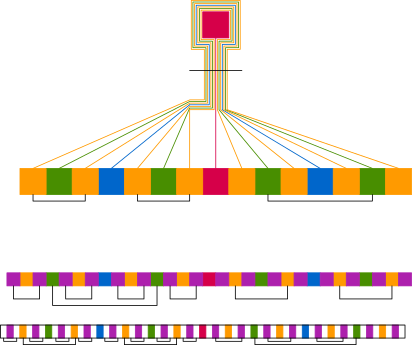
\includegraphics[width=400px]{Figures/entanglement.png}
%\caption{Old figure: A lower bound for $2^m$}
%\label{fig:convexprojection}
%\end{figure}

% section arbitrary (end)


\section{Conclusion} % (fold)
\label{sec:conclusion}

Open Questions that can be still researched:
\begin{enumerate}
	\item fat non-convex polygons for interesting fatness definitions. Because for some of them Theorem~\ref{thm:unbouded} holds.
	\item How about two polygons in the general setting? This would create an interesting comparison to either the one polygon or the three polygon cases where one is easy and one is unbounded.
	Solved reading: The Painter’s Problem: Covering a Grid with Colored Connected Polygons
	\item Can we give an algorithm for a stretch depending on the complexity of $A$, i.e., number of vertices, rotation number, \dots?
\end{enumerate}

% section conclusion (end)

\newpage
\appendix



\section{Write-up from Ivor for: Holes are Points}



Assume that all the holes are points. In that case we can create a pixel projection $B$ with a $\Theta(\sqrt[]{md})$ symmetrical Hausdorff distance to $A$. This projection is also used in the next section where regions are convex $\beta$-fat regions.  The lower bound for this variant is obtained in the following way: let there be $m$ holes in one pixel of diameter $d$. Then because the holes need to be disjoint, we need to expand all of $A$ by at least a factor $2\sqrt[]{m}d$ in both directions to allow each hole to have a single disjoint pixel.

\begin{figure}[H]
\centering
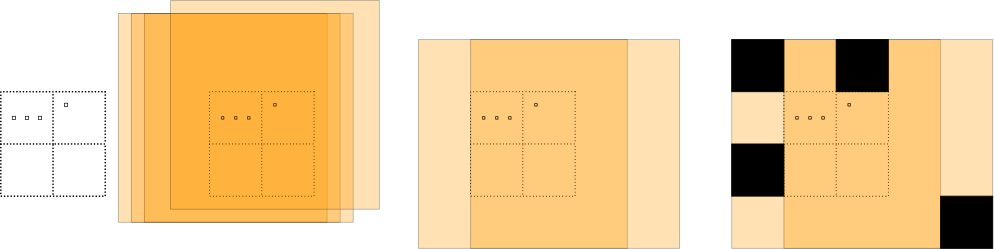
\includegraphics[width=300px]{Figures/pointprojection.png}
\caption{The four steps of the point projection $f$. Left we see $m=4$ points in two pixels with diameter $d$. The second frame shows all the non-translated regions $D_h$ with diameter $2\sqrt[]{m}d$. The third frame shows their translation, observe that holes in the same pixel always get assigned the same region $D_h$. The fourth frame shows an arbitrary assignment of holes to pixels in their regions.}
\label{fig:pointprojection}
\end{figure}


Given our object $A$ we can create a valid projection with a symmetrical Hausdorff distance to $B$ as follows: we assign to each hole $h \in H$ an axis-parallel square $D_h$ with diameter $2\sqrt[]{m}d$. We then align all the regions $D_h$ in the same way, in Figure \ref{fig:pointprojection} we align them to assign them to the left-bottom corner of each $D_h$ with the left-bottom corner of the pixel that contains the left-bottom corner of $D_h$. Lastly we iteratively assign each hole to a pixel in $D_h$ which is disjoint from any assigned pixel. There must always be such a pixel, because there are $4m$ pixels in each $D_h$ and there are only $m$ holes. This process gives a projection $f$ on $H$ with a symmetrical Hausdorff distance of at most $2\sqrt[]{m}d$ and Lemma \ref{lemma:expand} proves the rest.



\section{Write-up from Ivor for: Holes are Convex and Fat}



Recall that a region $B$ is $\beta$-fat if there exists an inscribed circle $I(B)$ and a enclosing circle $E(B)$ such that $\frac{|E(B)|}{|I(B)E} = \mathcal{O}(\beta)$.

Let the holes all be convex $\beta$-fat regions of arbitrary size. The projection for this case has a lower bound of $\Omega(\sqrt[]{m}d$ because the proof from the previous section can immediately be applied. The projection that realizes this lower bound borrows concepts from our previous projection. There we assigned to each region a ``super pixel'' $d_h$ with diameter $2\sqrt[]{m}d$. Instead of giving each hole a super pixel and aligning those with the grid, we first create aligned super pixels and assign our holes to those. We define $G$ be an arbitrary grid of super pixels $D$ with diameter $2\sqrt[]{m}d$ aligned with the pixel grid. 

\begin{observation}
\label{obs:covering}
Observe that if any hole $h \in H$ which is $\beta$-fat and convex has a diameter greater than $\mathcal{O}(\sqrt[]{h})$ then $h$ has to cover at least one super pixel in $G$. 
\end{observation}

\begin{figure}[H]
\centering
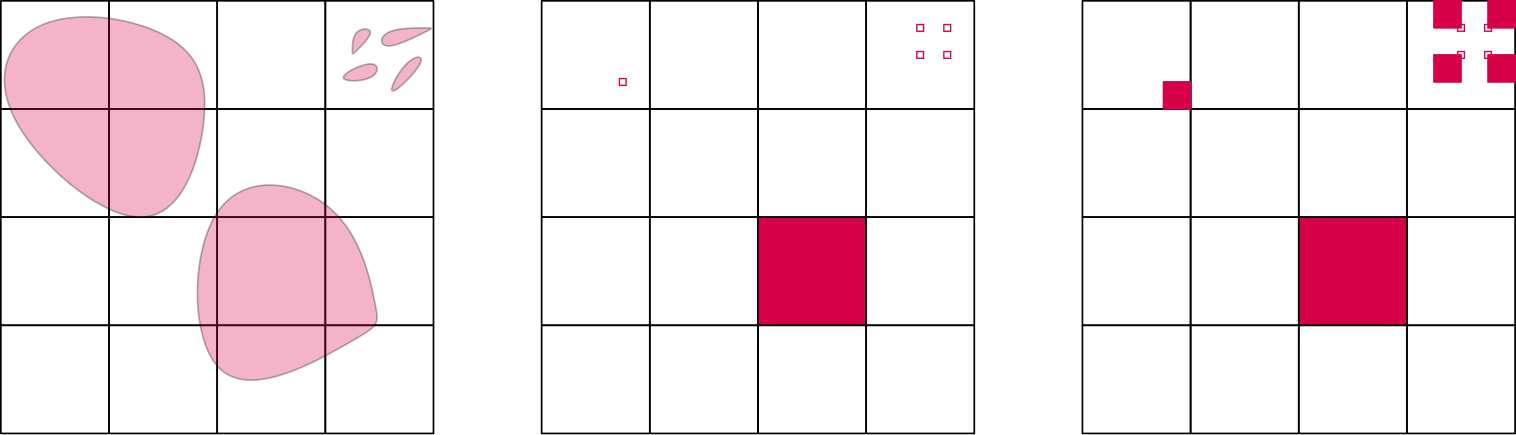
\includegraphics[width=300px]{Figures/fatprojection.png}
\caption{The four three steps of the $\beta$-fat projection $f$. Left we see $m=6$ $\beta$-fat holes in red and 16 super pixels with black borders. The middle figure is the projection $C$ where one region is collapsed to a super pixel and the remaining regions are collapsed to a point. The last figure shows the final projection $B$ where each remaining point is assigned a pixel which has a diameter which is $2\sqrt[]{6}$ times smaller than the super pixel. }
\label{fig:fatprojection}
\end{figure}


With this observation, we can make the following projection: if a hole $h$ covers at least one super pixel, we let $h$ cover all the super pixels that it covers. The remainder of their area we throw away and all the other regions get collapsed to their center point. Because of Observation \ref{obs:covering} this in-between-projection $C$ has a $\mathcal{O}(\sqrt[]{h}d)$ Hausdorff distance to $H$.
Just like in the previous section, we then assign each point to an arbitrary disjoint pixel in its super-pixel to create our valid projection $B$. The symmetric Hausdorff distance between $H$ and $C$ is $\mathcal{O}(\sqrt[]{h}d)$ and the distance $C$ and $B$ is $\mathcal{O}(\sqrt[]{h}d)$ so the symmetric Hausdorff distance between $H$ and $B$ must be $\mathcal{O}(\sqrt[]{h}d)$. See Figure \ref{fig:fatprojection} for an example.



\section{Write-up from Ivor for: Holes are Convex}



Let the holes have as their only requirement that they are convex. In that case we can immediately show that the projection has a lower-bound Hausdorff distance of $\Theta(md)$. The construction is shown in Figure \ref{fig:linesexample}. We would like to create a projection of any set of convex holes $H$ that implements this lower bound such that all the projected regions are orthoconvex.


\begin{figure}[H]
\centering

\includegraphics[width=20px]{Figures/linesexample.png}
\caption{The dotted square is a pixel with diameter $d$. We can let $m$ vertical lines intersect the pixel. If their length is far greater than $md$, we can only project these regions to $dm$ disjoint lines of pixels, which means that the outer lines must have a Hausdorff distance of $\Theta(md)$.}
\label{fig:linesexample}
\end{figure}


\begin{observation}
Let $h_1,h_2 \in H$ be two convex regions. If there exists a horizontal line segment $l_1$ which intersects $h_1$ and $h_2$ such that on $l_1$, $h_1$ is left from $h_2$ then there cannot be another horizontal line segment $l_2$ which intersects $h_1$ and $h_2$ such that on $l_2$, $h_1$ lies to the right of $h_2$. A symmetrical property holds for vertical line segments if we look at which segment is higher.
\end{observation}

To explain our orthoconvex projection, we first introduce some notation: the observation allows us to create a partial order $P_x$ and $P_y$ based on intersections with horizontal and vertical line segments respectively. Let $G$ be a grid of super pixels with diameter $2md+1$ that covers $H$, we denote a superpixel as $D \in G$. We define $X_H$ and $Y_H$ to be two indexes on $H$ that respect the partial orders $P_x$ and $P_y$ respectively. For any $D \in G$ we denote $D[x,y]$ to be the pixel in $D$ that is the $2x+1$'th from the left and the $2y+1'th$ pixel from the top. The algorithm involves assigning super pixels and pixels in $G$ to holes $h$ and in the end connecting those holes.

\begin{enumerate}
%\item If a hole $h$ covers at least one super pixel $D \in G$, we assign all $D$ which are coved by $h$ entirely to $h$.
%\item If a hole $h$ covers no super pixel, then for each super pixel $D$ which is intersected by $h$ we assign $D[X_H(h), Y_H(h)]$ to $h$.
\item For each super pixel $D$ which is intersected by a hole $h$ we assign $D[X_H(h), Y_H(h)]$ to $h$.
\item For all holes $h$, we connect all assigned pixels with a horizontal and vertical line. 
\item If a set of lines encloses a region, we fill that region.
\end{enumerate}


\begin{figure}[H]
\centering
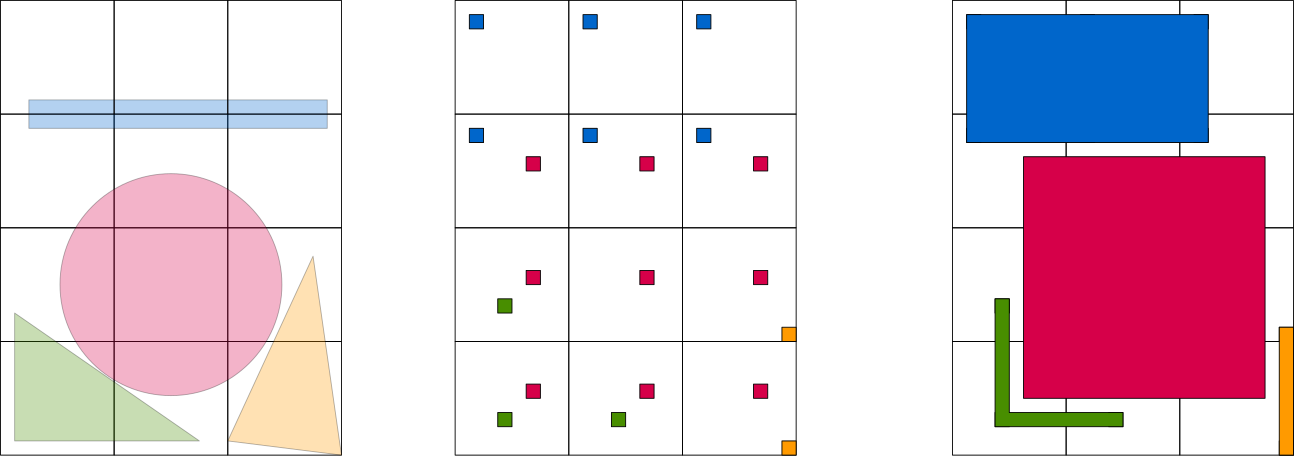
\includegraphics[width=400px]{Figures/convexprojection.png}
\caption{Four regions that intersect three times four super pixels and the four steps of our algorithm. four.}
\label{fig:convexprojection}
\end{figure}

The result is clearly orthoconvex, since all assigned pixels are connected with horizontal and vertical lines and all enclosed regions are filled in. The result must also be disjoint: Any region that originally intersected a region which was filled in step 4 must originally have been to the left/right top/bottom of the region that filled a hole and thus is projected left/right above/below the filled region.



\section{Write-up from Ivor for: Old Algorithm on How to Draw Arbitrary Polygons}



We obtain the upper bound via a construction where we iteratively insert the $h$ holes into a grid in an arbitrary order.
Fix an index on the holes: $H := \{ h_1, h_2 ... h_h \}$ and fix a 2-dimensional grid $G$ with cell diameter $ d 2^{h+1}$ over $A$.
For each grid cell $\hfill\pix$ we check which holes in $A$ intersect $\hfill\pix$ and we mark $\hfill\pix$ with these holes.

\begin{observation}
If in our projection each hole $h_i$ is a connected tree which spans all grid cells marked by $h_i$ then the symmetrical Hausdorff distance is $\Theta(d2^h)$.
\end{observation}

\begin{definition}[The iteration invariant]
In our proposed algorithm. After inserting hole $h_i$, every hole $h_j$ with $j \le i$ is a spanning tree. Where the tree has as least one vertex in each cell marked by $h_j$ and edges between vertices are orthogonal.
\end{definition}


Our algorithm works as follows: We start by inserting $h_1$ as an orthogonal MST of the center points of all its marked cells. This is clearly possible and it maintains the iteration invariant.



For all remained holes $h_i$ we do the following:

\paragraph*{Step 1}
We start by adding a (orthogonal) closed face around each hole $h_j$ with $j < i$ in the following way:
For each hole $h_j$ with $j < i$, for each edge $(a,b)$ we add four vertexes: $x_a, y_a, x_b, y_b$.  $x_a, x_b$ and $y_a,y_b$ are always connected with an orthogonal edge. If $a$ is a leaf, then $x_a,y_a$ are connected with an orthogonal edge and the same holds for $x_b,a_b$. Else per construction these edges are connected to another vertex. This creates an orthogonal face around each hole $h_j$.
Lastly we glue the holes together in the following way: For every pair of edges of $h_i$, if they are parallel, their endpoints pairwise end in the same grid and there is no edge in between, we identify then with one another. 

Each cell $\hfill\pix$ which is marked by $h_i$ and does not contain a vertex of $h_i$, we add a vertex of $h_i$ and we name these vertexes \emph{champions}. In the original drawing $\hfill\pix$ was intersected by $h_i$ and connected. This in particular means that at least one edge of $\hfill\pix$ was intersected by $h_1$. For these edges we add an orthogonal edge from the champion to the cell that shares the edge with $\hfill\pix$. The result is that $h_i$ is connected and that there is a vertex in each cell marked by $h_i$.
note that after step 1. The iteration invariant holds for all holes $h_j$ with $j < i$ but not for $h_i$. See Figure \ref{fig:cycle} for an example.

\begin{figure}[H]
\centering
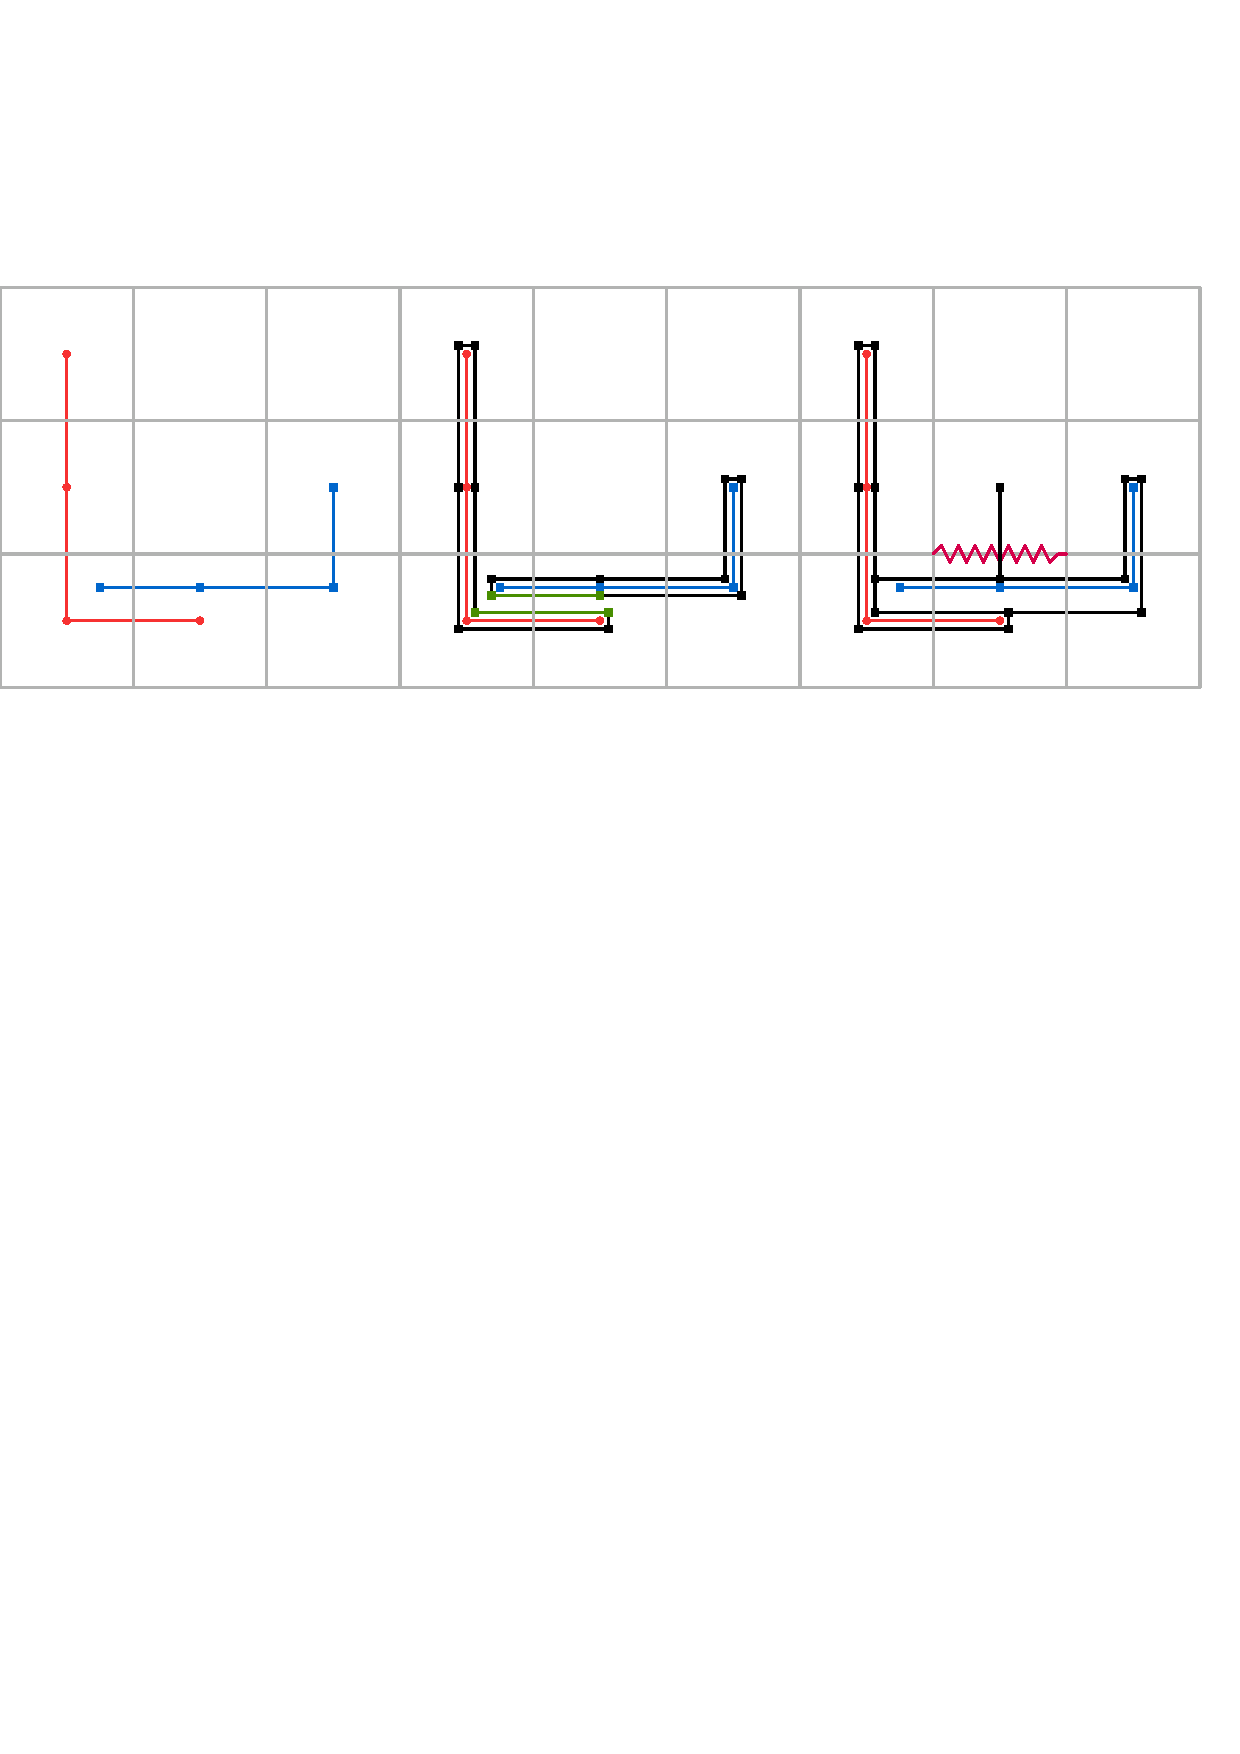
\includegraphics[page = 1]{Figures/cycle.pdf}
\caption{Left we see the result after inserting $h_1$ and $h_2$ in red and blue respectively. In the middle we see the two orthogonal cycles around $h_1$ and $h_2$. Note that the green edges can be identified to one another. The edge connected straight to the right is no candidate for gluing because the endpoints do not end in the same grid cells, so we get an extra }
\label{fig:cycle}
\end{figure}

\paragraph*{Step 2.}

In step 2. We delete all endpoints of $h_i$ which are in a cell that is not marked by $h_i$. We also delete all edges with less than 2 endpoints. All remaining vertices $x$ which used to have an outgoing edge and have lost it are marked \emph{broken.}

$h_i$ is now a collection of curves with three types of edges:

\begin{itemize}
\item Edges where all endpoints are regular (these are in the interior of a path). We call these \emph{regular edges}
\item Edges which end in a champion. We call these \emph{champion edges}
\item The case where at least one or two broken endpoints are involved but no champions. We call these \emph{broken edges}
\end{itemize}


\begin{observation}
after the gluing, each of $h_i$ is in at most 2 cycles.
\end{observation}
\paragraph*{Step 3.}

\begin{figure}[H]
\centering
\includegraphics[page = 2]{Figures/cycle.pdf}
\caption{ }
\label{fig:cycle2}
\end{figure}

\end{document}
